\newpage
\section{Introduction}
Road vehicles typically use a hydraulic brake system for the brakes, however future road vehicles are expected to have this replaced with a brake-by-wire system. In a brake-by-wire system, shown in Figure 1 below, the brake pedal is connected to a central unit (CU). The central unit sends messages with brake commands to each of the four wheel units (WU). In addition, two serial busses (SB1 and SB2) are used for data communication. Furthermore, to improve the brake performance of the system, the system uses an anti-lock-braking algorithm for each wheel. The anti-lock program receives input in the form of current wheel speed and brake force commands generated by a stability control program, which is executed in the central unit of the system.  The advantages of using a brake-by-wire system compared to the more traditional hydraulic brake systems is a lower cost, weight and a more simple integration with other stability control and active safety systems.\\
\\
This report contains the results from analysing two different design architectures for the brake-by-wire system with the help of dependability modeling, in order to determine which one is more reliable and the various advantages and disadvantages for the two architectures. The report starts with a detailed description of the two architectures and the various models used in the brake-by-wire system. Such as the wheel units and central unit. The report then proceeds to the results from the analysis followed by the discussion of the result and what conclusions that can be made.

\begin{figure}[h!]
  \centering
  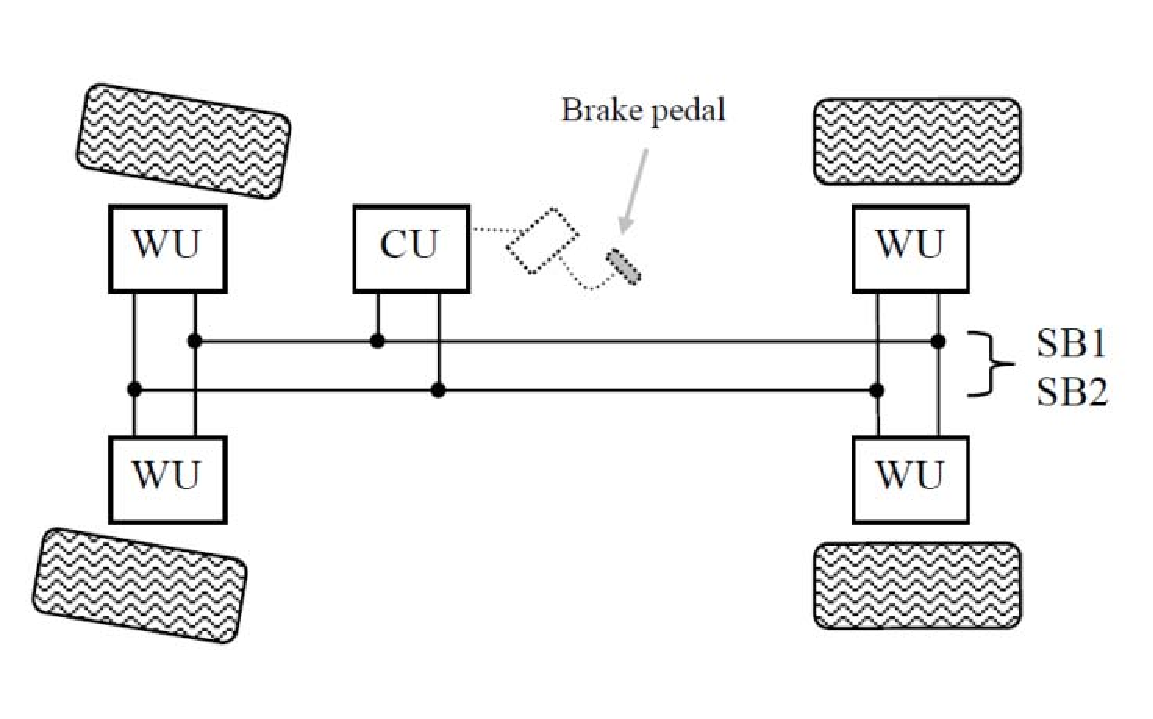
\includegraphics[scale=.5]{Fig1.pdf}
  \caption{Brake-by-wire system}
  \label{fig1}
\end{figure}